\documentclass{article}

% packages
  % basic stuff for rendering math
  \usepackage[letterpaper, top=1in, bottom=1in, left=1in, right=1in]{geometry}
  \usepackage[utf8]{inputenc}
  \usepackage[english]{babel}
  \usepackage{amsmath} 
  \usepackage{amssymb}
  % \usepackage{amsthm}

  % extra math symbols and utilities
  \usepackage{mathtools}        % for extra stuff like \coloneqq
  \usepackage{mathrsfs}         % for extra stuff like \mathsrc{}
  \usepackage{centernot}        % for the centernot arrow 
  \usepackage{bm}               % for better boldsymbol/mathbf 
  \usepackage{enumitem}         % better control over enumerate, itemize
  \usepackage{hyperref}         % for hypertext linking
  \usepackage{fancyvrb}          % for better verbatim environments
  \usepackage{newverbs}         % for texttt{}
  \usepackage{xcolor}           % for colored text 
  \usepackage{listings}         % to include code
  \usepackage{lstautogobble}    % helper package for code
  \usepackage{parcolumns}       % for side by side columns for two column code
  

  % page layout
  \usepackage{fancyhdr}         % for headers and footers 
  \usepackage{lastpage}         % to include last page number in footer 
  \usepackage{parskip}          % for no indentation and space between paragraphs    
  \usepackage[T1]{fontenc}      % to include \textbackslash
  \usepackage{footnote}
  \usepackage{etoolbox}

  % for custom environments
  \usepackage{tcolorbox}        % for better colored boxes in custom environments
  \tcbuselibrary{breakable}     % to allow tcolorboxes to break across pages

  % figures
  \usepackage{pgfplots}
  \pgfplotsset{compat=1.18}
  \usepackage{float}            % for [H] figure placement
  \usepackage{tikz}
  \usepackage{tikz-cd}
  \usepackage{circuitikz}
  \usetikzlibrary{arrows}
  \usetikzlibrary{positioning}
  \usetikzlibrary{calc}
  \usepackage{graphicx}
  \usepackage{algorithmic}
  \usepackage{caption} 
  \usepackage{subcaption}
  \captionsetup{font=small}

  % for tabular stuff 
  \usepackage{dcolumn}

  \usepackage[nottoc]{tocbibind}
  \pdfsuppresswarningpagegroup=1
  \hfuzz=5.002pt                % ignore overfull hbox badness warnings below this limit

% New and replaced operators
  \DeclareMathOperator{\Tr}{Tr}
  \DeclareMathOperator{\Sym}{Sym}
  \DeclareMathOperator{\Span}{span}
  \DeclareMathOperator{\std}{std}
  \DeclareMathOperator{\Cov}{Cov}
  \DeclareMathOperator{\Var}{Var}
  \DeclareMathOperator{\Corr}{Corr}
  \DeclareMathOperator{\pos}{pos}
  \DeclareMathOperator*{\argmin}{\arg\!\min}
  \DeclareMathOperator*{\argmax}{\arg\!\max}
  \newcommand{\ket}[1]{\ensuremath{\left|#1\right\rangle}}
  \newcommand{\bra}[1]{\ensuremath{\left\langle#1\right|}}
  \newcommand{\braket}[2]{\langle #1 | #2 \rangle}
  \newcommand{\qed}{\hfill$\blacksquare$}     % I like QED squares to be black

% Custom Environments
  \newtcolorbox[auto counter, number within=section]{question}[1][]
  {
    colframe = orange!25,
    colback  = orange!10,
    coltitle = orange!20!black,  
    breakable, 
    title = \textbf{Question \thetcbcounter ~(#1)}
  }

  \newtcolorbox[auto counter, number within=section]{exercise}[1][]
  {
    colframe = teal!25,
    colback  = teal!10,
    coltitle = teal!20!black,  
    breakable, 
    title = \textbf{Exercise \thetcbcounter ~(#1)}
  }
  \newtcolorbox[auto counter, number within=section]{solution}[1][]
  {
    colframe = violet!25,
    colback  = violet!10,
    coltitle = violet!20!black,  
    breakable, 
    title = \textbf{Solution \thetcbcounter}
  }
  \newtcolorbox[auto counter, number within=section]{lemma}[1][]
  {
    colframe = red!25,
    colback  = red!10,
    coltitle = red!20!black,  
    breakable, 
    title = \textbf{Lemma \thetcbcounter ~(#1)}
  }
  \newtcolorbox[auto counter, number within=section]{theorem}[1][]
  {
    colframe = red!25,
    colback  = red!10,
    coltitle = red!20!black,  
    breakable, 
    title = \textbf{Theorem \thetcbcounter ~(#1)}
  } 
  \newtcolorbox[auto counter, number within=section]{proposition}[1][]
  {
    colframe = red!25,
    colback  = red!10,
    coltitle = red!20!black,  
    breakable, 
    title = \textbf{Proposition \thetcbcounter ~(#1)}
  } 
  \newtcolorbox[auto counter, number within=section]{corollary}[1][]
  {
    colframe = red!25,
    colback  = red!10,
    coltitle = red!20!black,  
    breakable, 
    title = \textbf{Corollary \thetcbcounter ~(#1)}
  } 
  \newtcolorbox[auto counter, number within=section]{proof}[1][]
  {
    colframe = orange!25,
    colback  = orange!10,
    coltitle = orange!20!black,  
    breakable, 
    title = \textbf{Proof. }
  } 
  \newtcolorbox[auto counter, number within=section]{definition}[1][]
  {
    colframe = yellow!25,
    colback  = yellow!10,
    coltitle = yellow!20!black,  
    breakable, 
    title = \textbf{Definition \thetcbcounter ~(#1)}
  } 
  \newtcolorbox[auto counter, number within=section]{example}[1][]
  {
    colframe = blue!25,
    colback  = blue!10,
    coltitle = blue!20!black,  
    breakable, 
    title = \textbf{Example \thetcbcounter ~(#1)}
  } 
  \newtcolorbox[auto counter, number within=section]{code}[1][]
  {
    colframe = green!25,
    colback  = green!10,
    coltitle = green!20!black,  
    breakable, 
    title = \textbf{Code \thetcbcounter ~(#1)}
  } 
  \newtcolorbox[auto counter, number within=section]{algo}[1][]
  {
    colframe = green!25,
    colback  = green!10,
    coltitle = green!20!black,  
    breakable, 
    title = \textbf{Algorithm \thetcbcounter ~(#1)}
  } 

  \BeforeBeginEnvironment{example}{\savenotes}
  \AfterEndEnvironment{example}{\spewnotes}
  \BeforeBeginEnvironment{lemma}{\savenotes}
  \AfterEndEnvironment{lemma}{\spewnotes}
  \BeforeBeginEnvironment{theorem}{\savenotes}
  \AfterEndEnvironment{theorem}{\spewnotes}
  \BeforeBeginEnvironment{corollary}{\savenotes}
  \AfterEndEnvironment{corollary}{\spewnotes}
  \BeforeBeginEnvironment{proposition}{\savenotes}
  \AfterEndEnvironment{proposition}{\spewnotes}
  \BeforeBeginEnvironment{definition}{\savenotes}
  \AfterEndEnvironment{definition}{\spewnotes}
  \BeforeBeginEnvironment{exercise}{\savenotes}
  \AfterEndEnvironment{exercise}{\spewnotes}
  \BeforeBeginEnvironment{proof}{\savenotes}
  \AfterEndEnvironment{proof}{\spewnotes}
  \BeforeBeginEnvironment{solution}{\savenotes}
  \AfterEndEnvironment{solution}{\spewnotes}
  \BeforeBeginEnvironment{question}{\savenotes}
  \AfterEndEnvironment{question}{\spewnotes}
  \BeforeBeginEnvironment{code}{\savenotes}
  \AfterEndEnvironment{code}{\spewnotes}
  \BeforeBeginEnvironment{algo}{\savenotes}
  \AfterEndEnvironment{algo}{\spewnotes}

  \definecolor{dkgreen}{rgb}{0,0.6,0}
  \definecolor{gray}{rgb}{0.5,0.5,0.5}
  \definecolor{mauve}{rgb}{0.58,0,0.82}
  \definecolor{darkblue}{rgb}{0,0,139}
  \definecolor{lightgray}{gray}{0.93}
  \renewcommand{\algorithmiccomment}[1]{\hfill$\triangleright$\textcolor{blue}{#1}}

  % default options for listings (for code)
  \lstset{
    autogobble,
    frame=ltbr,
    language=C, 
    aboveskip=3mm,
    belowskip=3mm,
    showstringspaces=false,
    columns=fullflexible,
    keepspaces=true,
    basicstyle={\small\ttfamily},
    numbers=left,
    firstnumber=1,                        % start line number at 1
    numberstyle=\tiny\color{gray},
    keywordstyle=\color{blue},
    commentstyle=\color{dkgreen},
    stringstyle=\color{mauve},
    backgroundcolor=\color{lightgray}, 
    breaklines=true,                      % break lines
    breakatwhitespace=true,
    tabsize=3, 
    xleftmargin=2em, 
    framexleftmargin=1.5em, 
    stepnumber=1
  }

% Page style
  \pagestyle{fancy}
  \fancyhead[L]{JavaScript}
  \fancyhead[C]{Muchang Bahng}
  \fancyhead[R]{Fall 2024} 
  \fancyfoot[C]{\thepage / \pageref{LastPage}}
  \renewcommand{\footrulewidth}{0.4pt}          % the footer line should be 0.4pt wide
  \renewcommand{\thispagestyle}[1]{}  % needed to include headers in title page

\begin{document}

\title{JavaScript}
\author{Muchang Bahng}
\date{Fall 2024}

\maketitle
\tableofcontents
\pagebreak

\section{Events} 
  
  There are many events that we can handle. Say that we have an event \texttt{event}. Then, upon this event, we can have it call some JavaScript code of the form. 
  \begin{lstlisting}
    <p id="paragrpah" event="function()"></p>
  \end{lstlisting}

  If we think of each tag as an object, these events are really attributes of this object that point to JS functions. 
 
  \begin{example}[Significant Events]
    It's worth mentioning a couple events that are important. 
    \begin{enumerate}
      \item \texttt{onclick}. When a user clicks on something. 
      \item \texttt{onload}. When a tag loads. 
      \item \texttt{onerror}. When a tag fails to load.  
      \item \texttt{onkeydown}. When a key is pressed down. 
    \end{enumerate}
  \end{example}

\section{Asynchronous Handling}

  Let's talk about the architecture of the JavaScript runtime environment, which has a bit more components than that of other languages like C or Python. This allows better handling of asynchronous code and provides additional objects by the browser.  

  \begin{definition}[JavaScript Runtime Environment]
    It contains the following. 
    \begin{enumerate}
      \item The \textit{JavaScript Engine} consists of the \textit{stack} and the \textit{heap} handles function calls and allows access to larger pools of memory, respectively. 
      \item The \textit{Web/Browser API}, separate fro the JS Engine, can be communicated with using JS, enabling us to do things concurrently outside of the JS interpreter. The language itself is single-threaded, but the browser APIs act as separate threads. Callback functions from the API is sent to the task queue.   
      \item The \textit{callback/task queue} is a message queue where each message has an associated function to be called. After the call stack is emptied, during the Event Loop, runtime handles the first message in the queue by callings its functions and popping them onto to the call stack. 
      \item The \textit{Microtask queue} is a higher priority of the task queue and handles Microtasks callbacks. 
      \item The \textit{event loop} constantly checks whether or not the call stack is empty. When the call stack is empty, all queued up microtasks from this queue are popped onto the call stack. If both the call stack and the microtask queue are empty, the event loops dequeues tasks from the task queue and calls them. 
    \end{enumerate}

    \begin{figure}[H]
      \centering 
      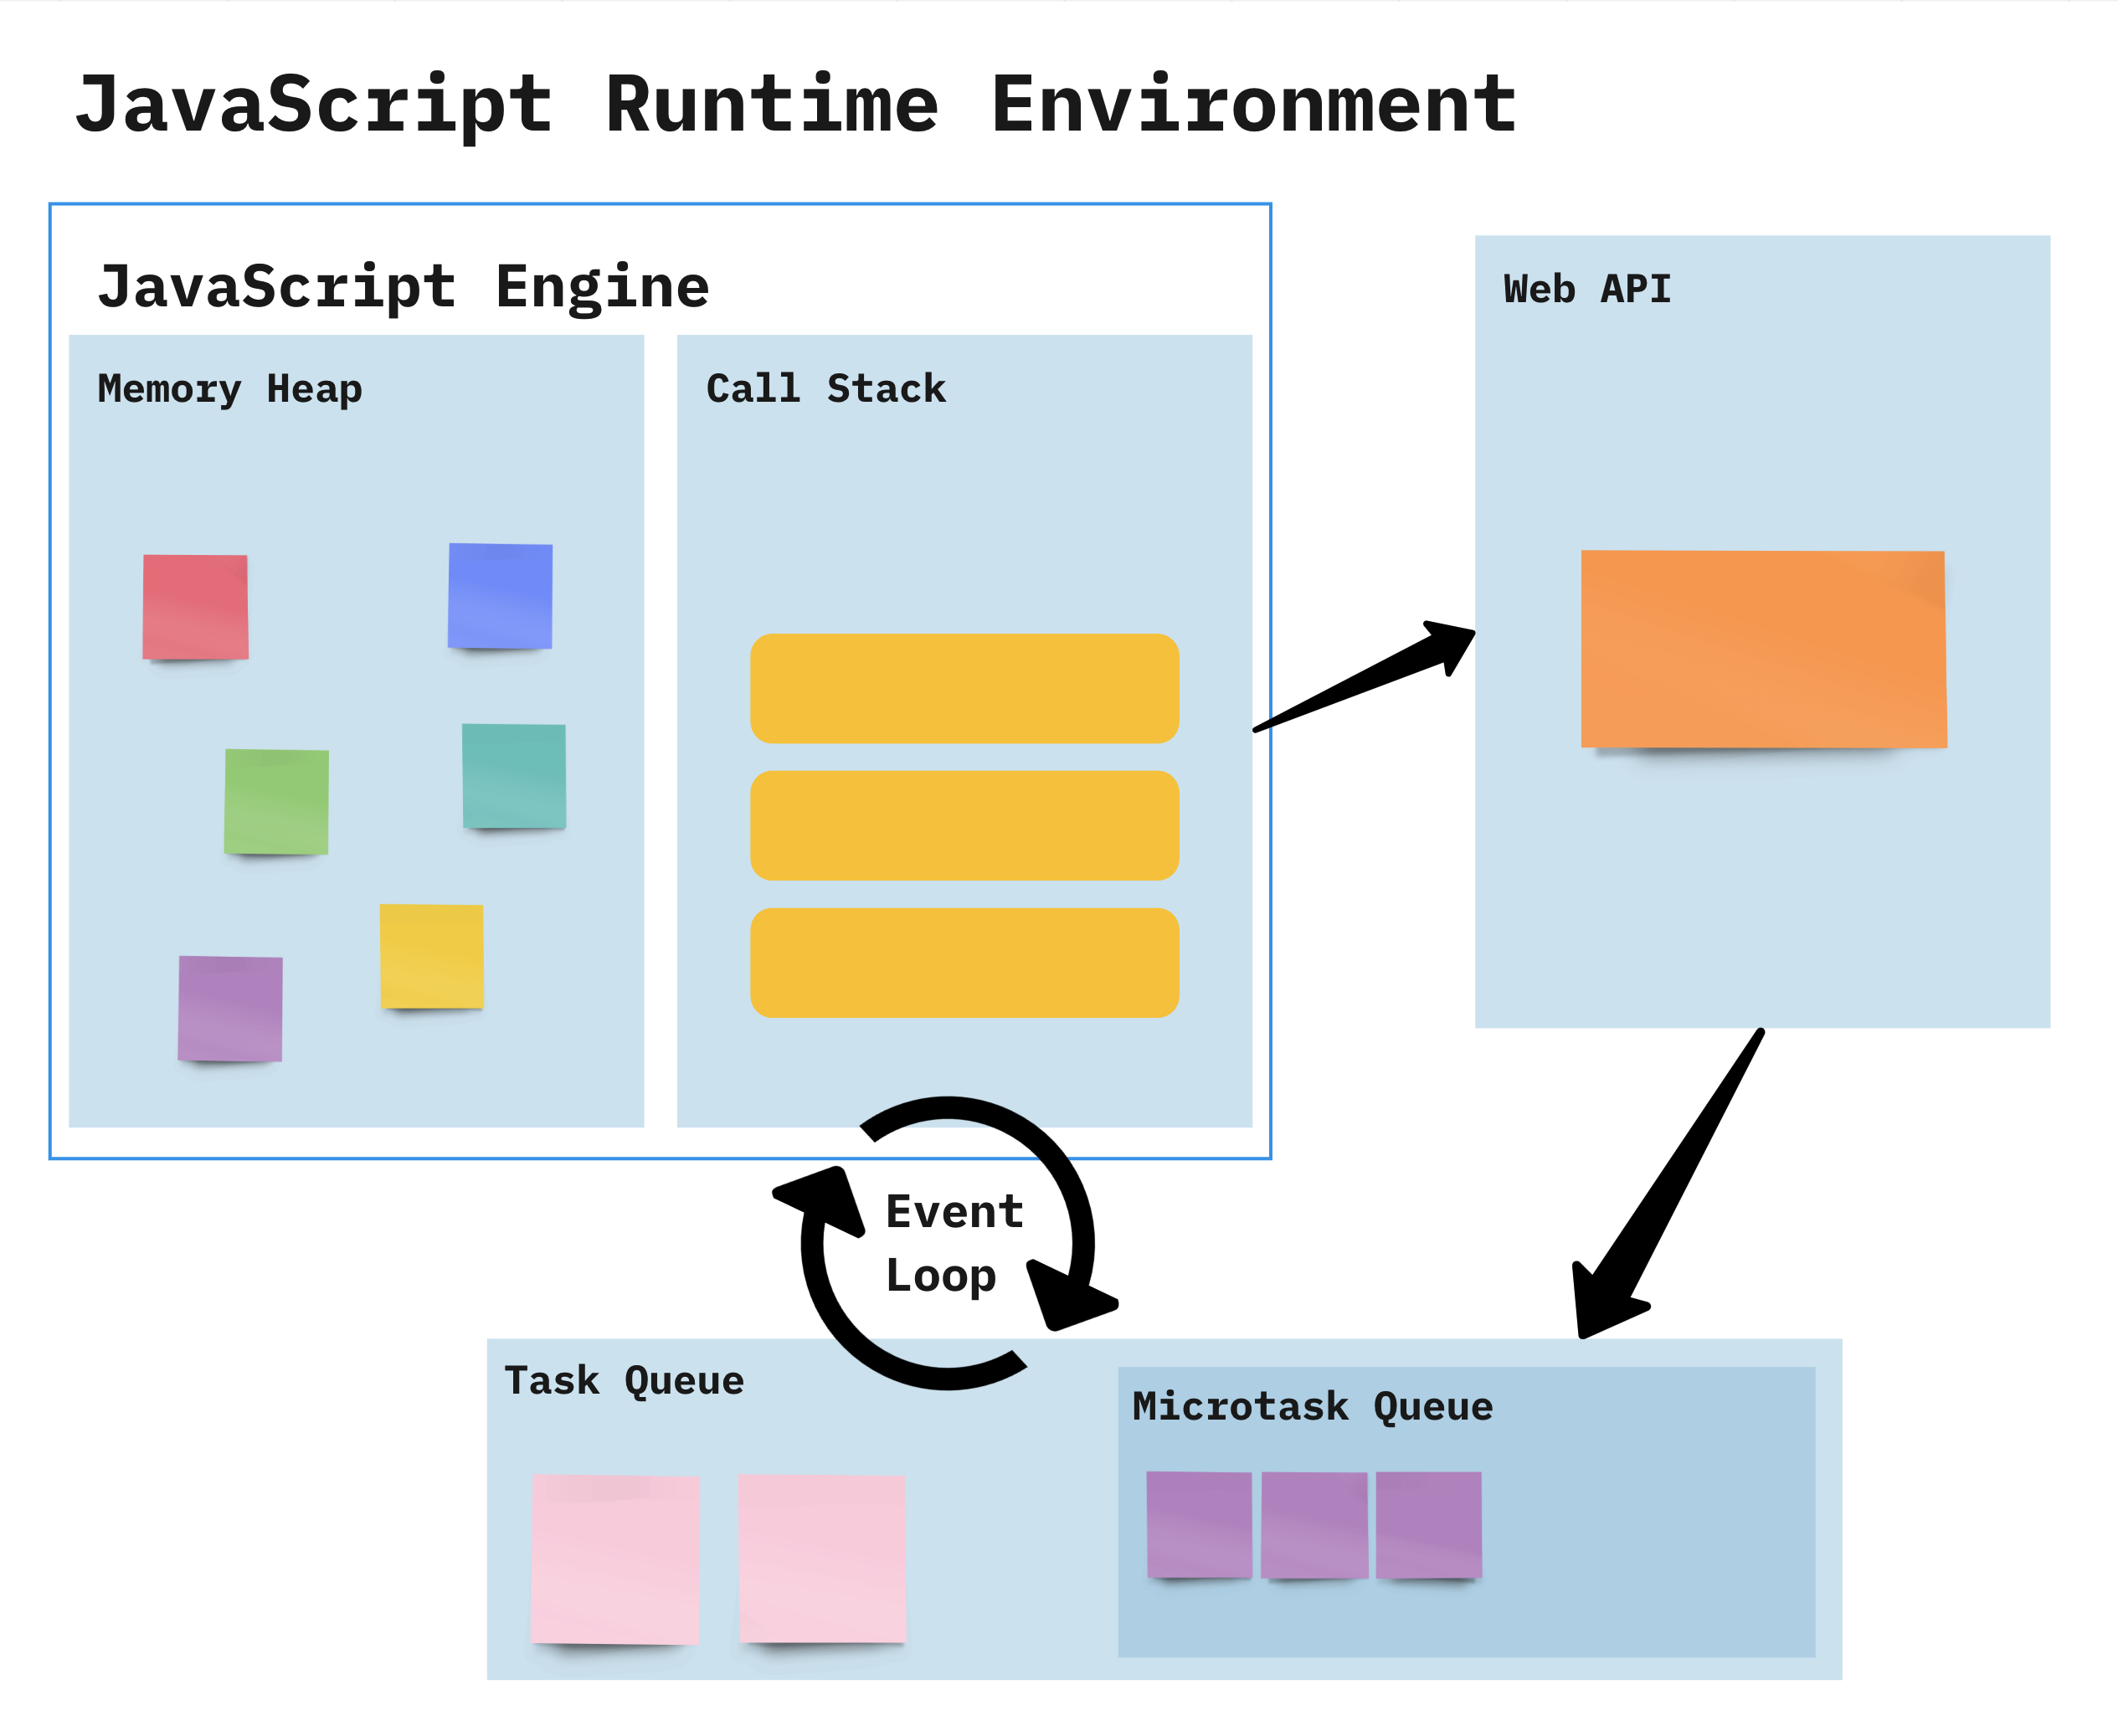
\includegraphics[scale=0.2]{img/js_runtime_env.png}
      \caption{The JS runtime environment contains task queues, the Web API, and the event handler.} 
      \label{fig:js_runtime_env}
    \end{figure}
  \end{definition}

  Three common functions in the web API are 
  \begin{enumerate}
    \item \texttt{setTimeout(function, ms)}, which delays the call of a function by \texttt{ms} milliseconds. 
    \item \texttt{setInterval(function, ms)}, which repeats the call of a function every \texttt{ms} milliseconds. 
    \item \texttt{addEventListener(type, listener)}, which adds a listener that scans for some event, e.g. a mouse click, scroll, hover, etc. 
  \end{enumerate}

  In the regular call stack, we can already see that calling these functions will just stop everything. \texttt{setTimeout} will stop everything for some time before its argument function is called, and an event listener will repeatedly call some function to detect an event, overflowing the stack.  

  \subsection{Callback Functions}

    \begin{definition}[Callback Function]
      A \textbf{callback function} is a function that is passed as an argument to another function and is executed at the completion of that function. 
    \end{definition}

    This is useful since it guarantees that asynchronous tasks that gets moved to the web API is called. 

    \begin{definition}[Callback Hell]
      At some points,
    \end{definition}

  \subsection{Promises}

    \begin{definition}[Promise]
      A \texttt{Promise} object is a wrapper around a (HTTP) request. It has the following attributes. 
      \begin{enumerate}
        \item \texttt{PromiseState} starts off as \texttt{pending} as we request the packet, and then depending on if it successfully retrieved the data (called \textit{resolved}) or not, it updates to \texttt{OK} or \texttt{ERR}. 
        \item \texttt{PromiseResult} 
        \item \texttt{PromiseFulfillReactions}
        \item \texttt{PromiseRejectReactions}
        \item \texttt{PromiseIsHandled} 
      \end{enumerate}
      
      It is constructed with a function that takes in two arguments. 
      \begin{enumerate}
        \item A \texttt{resolve} function that is called when the promise is successful. When \texttt{resolve(val)} is called, \texttt{val} is stored in \texttt{PromiseResult}. 
        \item A \texttt{reject} function that is called when the promise is unsuccessful. When \texttt{reject(val)} is called, \texttt{val} is stored in \texttt{PromiseResult}.  
      \end{enumerate}
    \end{definition}

    \begin{example}[Resolve without Asynchronous Functions]
      A trivial promise object is constructed that calls \texttt{resolve} or \texttt{reject}. 

      \noindent\begin{minipage}{.5\textwidth}
      \begin{lstlisting}[]{Code}
        let p = new Promise(
          function(resolve, reject) {
            resolve(1); 
          }
        )
        console.log(p); 

        Promise {
          1,
          [Symbol(async_id_symbol)]: 28,
          [Symbol(trigger_async_id_symbol)]: 6
        }
        .
        .
      \end{lstlisting}
      \end{minipage}
      \hfill
      \begin{minipage}{.49\textwidth}
      \begin{lstlisting}[]{Output}
        let p = new Promise(
          function(resolve, reject) {
            reject("bruh"); 
          }
        )

        console.log(p); 
        Promise {
          <rejected> 'bruh',
          [Symbol(async_id_symbol)]: 29,
          [Symbol(trigger_async_id_symbol)]: 6
        }
        undefined
        Uncaught 'bruh'
      \end{lstlisting}
      \end{minipage}
    \end{example}

  \subsection{Then, Catch, Finally}

    A \texttt{Promise} object has three methods that tells us how to \textit{react} depending on the value of \texttt{PromiseResult}, and it ends up returning a \textit{new} Promise object with its own \texttt{PromiseResult} attribute being what was returned by the method. 
    \begin{enumerate}
      \item \texttt{then} is used to react mainly to successful resolves and sometimes to errors. \texttt{then(f, g)} will call \texttt{f(PromiseResult)} when the promise is resolved and \texttt{g(PromiseResult)} if not. 
        It takes two arguments: 

      \item \texttt{catch} is used to resolve errors, which takes in one argument that will be called with \texttt{PromiseResult} when it is rejected. \texttt{catch(g)} will call \texttt{g(PromiseResult)} upon error. It can be used multiple times and in between \texttt{then} handlers, so when a promise rejects, the control jumpt to the closest rejection handler. 

      \item \texttt{finally} is used as a cleanup method and is always called. \texttt{finally(f)} is equivalent to \texttt{then(f, f)}.  
    \end{enumerate}


    \begin{example}
      Here is an example of how we use then statements. 
      
      \noindent\begin{minipage}{.5\textwidth}
      \begin{lstlisting}[]{Code}
        let promise = new Promise(
          function(resolve, reject) {
            setTimeout(
              () => resolve("done!"), 1000
            );
          }
        );
        // resolve runs 1st function in .then
        promise.then(
          // shows "done!" after 1 second
          result => alert(result), 
          // doesn't run
          error => alert(error) 
        );
      \end{lstlisting}
      \end{minipage}
      \hfill
      \begin{minipage}{.49\textwidth}
      \begin{lstlisting}[]{Output}
        let promise = new Promise(
          function(resolve, reject) {
            setTimeout(() => reject(
              new Error("Whoops!")), 1000
            );
          }
        );
        // reject runs 2nd function in .then
        promise.then(
          // doesn't run
          result => alert(result), 
          // "Error: Whoops!" after 1 sec 
          error => alert(error) 
        ); 
      \end{lstlisting}
      \end{minipage}
    \end{example}

    Since calling a bunch of \texttt{then}'s gives us a new Promise, we can chain them together to get a bunch of promises. Check this out. 

    \begin{lstlisting}
      new Promise(function(resolve, reject) {

        setTimeout(() => resolve(1), 1000); // (*)

      }).then(function(result) { // (**)

        alert(result); // 1
        return result * 2;

      }).then(function(result) { // (***)

        alert(result); // 2
        return result * 2;

      }).then(function(result) {

        alert(result); // 4
        return result * 2;

      });
    \end{lstlisting}

    \begin{enumerate}
      \item The initial promise is resolved with a value of 1. 
      \item The \texttt{then} handler creates a new promise resolved with value 2. 
      \item the next \texttt{then} handler creates a new promise with value 4. 
    \end{enumerate}

    Since we have a bunch of alert calls, we will be alerted with values of 1, 2, and 4. Rather than returning a bunch of numbers we can also return the promise object itself. The following code is equivalent, but with a 1 second delay in between. 

    \begin{lstlisting}
      new Promise(function(resolve, reject) {

        setTimeout(() => resolve(1), 1000);

      }).then(function(result) {

        alert(result); // 1

        return new Promise((resolve, reject) => { // (*)
          setTimeout(() => resolve(result * 2), 1000);
        });

      }).then(function(result) { // (**)

        alert(result); // 2

        return new Promise((resolve, reject) => {
          setTimeout(() => resolve(result * 2), 1000);
        });

      }).then(function(result) {

        alert(result); // 4

      });
    \end{lstlisting}`

    Note that a classic newbie error is that the following is not promise chaining, as it produces alerts 1, 1, and 1. 

    \begin{lstlisting}
      let promise = new Promise(function(resolve, reject) {
        setTimeout(() => resolve(1), 1000);
      });

      promise.then(function(result) {
        alert(result); // 1
        return result * 2;
      });

      promise.then(function(result) {
        alert(result); // 1
        return result * 2;
      });

      promise.then(function(result) {
        alert(result); // 1
        return result * 2;
      });
    \end{lstlisting}

    This is because we are just adding several handlers to one promise, and so we are not taking the new promise returned from the previous handler into the next handler. 

    \begin{example}[Quotes API]
      Let's use this to process some quotes. We call fetch on some API url, which returns a promise object. I use the \texttt{then} handler to call a function that first preprocesses the promise result into a json format. Once this is done, I call another function to print this json data. If any of these don't work, i.e. the Promise calls the \texttt{reject} function, then there is a catch statement to log the error. 
      \begin{lstlisting}
        let p = fetch("https://zenquotes.io/api/random")
          .then((resolve) => resolve.json())
          .then((data) => console.log(data))
          .catch((err) => console.log(err)); 

        ... 
        [
          {
            q: 'Happiness is a gift and the trick is not...', 
            a: 'Charles Dickens',
            h: '<blockquote>&ldquo;Happiness is a gift and...'
          }
        ]
        
      \end{lstlisting}
    \end{example}

    We have just added one catch statement so far to handle all errors. However, the errors could come in any link of the Promise chain. For example, 
    \begin{enumerate}
      \item We may not be able to retrieve the data from the network. 
      \item The data format may not be in json. 
      \item Some downstream postprocessing could be corrupted. 
    \end{enumerate}

  \subsection{Promise API}

    There are some static methods in the \texttt{Promise} class that are useful to know. 

    \begin{definition}[\texttt{Promise.all}]
      If we want many promises to execute in parallel and wait until all of them are ready, we can use \texttt{Promise.all}, which wraps all promises into a single \texttt{Promise} object. It takes an iterable (usually an array of promises) and returns a new promise. 
      
      \begin{lstlisting}
        let promise = Promise.all(iterable); 
      \end{lstlisting}

      If any of the promises are rejected, the promise returned by \texttt{Promise.all} immediately rejects with that error and forgets about all the resolved ones. 
    \end{definition}

    \begin{example}
      The wrapper is handled with the alert function, which will return $1, 2, 3$, in the order of the elements of the array, regardless of the time it takes to complete. 
      
      \begin{lstlisting}
        Promise.all([
          new Promise(resolve => setTimeout(() => resolve(1), 3000)), // 1
          new Promise(resolve => setTimeout(() => resolve(2), 2000)), // 2
          new Promise(resolve => setTimeout(() => resolve(3), 1000))  // 3
        ]).then(alert); // 1,2,3  
      \end{lstlisting}

      A slightly more practical example is if we want to fetch an array of URLs. 

      \begin{lstlisting}
        let urls = [
          'https://api.github.com/users/iliakan',
          'https://api.github.com/users/remy',
          'https://api.github.com/users/jeresig'
        ];

        // map every url to the promise of the fetch
        let requests = urls.map(url => fetch(url));

        // Promise.all waits until all jobs are resolved
        Promise.all(requests)
          .then(responses => responses.forEach(
            response => alert(`${response.url}: ${response.status}`)
          )); 
      \end{lstlisting}
    \end{example}

    Notice that \texttt{Promise.all} can be wasteful since if we resolve in all Promises except one, all Promises are lost. This is good for all or nothing cases, but sometimes, we just want a simple wrapper. This is where allSettled comes in. 

    \begin{definition}[\texttt{Promises.allSettled}]
      \texttt{Promises.allSettled} waits for all promises to settle, regardless of the result and gives an array of form 
      \begin{enumerate}
        \item \texttt{\{status:"fulfilled", value:result\}} for successful responses, 
        \item \texttt{\{status:"rejected", reason:error\}} for errors
      \end{enumerate}
      Its syntax is: 
      \begin{lstlisting}
        let promise = Promise.allSettled(iterable); 
      \end{lstlisting}
    \end{definition}

    \begin{definition}[\texttt{Promise.race}]
      \texttt{Promise.race} is similar to \texttt{Promise.all}, but waits only for the first settled promise and gets its result (or error). 
      \begin{lstlisting}
        let promise = Promise.race(iterable); 
      \end{lstlisting}
    \end{definition}

    \begin{definition}[\texttt{Promise.any}]
      \texttt{Promise.any} is similar to \texttt{Promise.race}, but waits only for the first \textit{successful} settled promise and gets its result. 
      \begin{lstlisting}
        let promise = Promise.any(iterable); 
      \end{lstlisting}
      If all promises are rejected, then the returned promise is rejected with \texttt{AggregateError}. 
    \end{definition}


    \begin{definition}[\texttt{Promise.resolve}/\texttt{Promise.reject}]
      The following two class methods are mostly obsolete due to the \texttt{async/await} syntax, but we'll cover it here. 
      \begin{enumerate}
        \item \texttt{Promise.resolve(value)} creates a resolved promise with the result \texttt{value}. It is the same as 
        \begin{lstlisting}
          let promise = new Promise(resolve => resolve(value));
        \end{lstlisting}
        It is used when a function is expected to return a promise.

        \item \texttt{Promise.reject(error)} creates a rejected promise with error \texttt{error}. It is the same as 
        \begin{lstlisting}
          let promise = new Promise((resolve, reject) => reject(error));
        \end{lstlisting}
      \end{enumerate}
    \end{definition}

  \subsection{Async and Await}

    We already have the tools and knowledge required to learn about async and await, which is just simpler syntax for handling Promises. 

    \begin{definition}[\texttt{async}]
      The \texttt{async} keyword, which can be put before a function, indicates two things: 
      \begin{enumerate}
        \item The function will run asynchronously via the JavaScript's event loop. This means that its simply running on another thread, independent of the main call stack, or more specifically, it is run asynchronously through the web API which is then pushed into the task queue.   
        \item Its returned object will be a \texttt{Promise} object with a result of whatever it returns. So it ensures that the function returns a promise and wraps non-promises in it. 
      \end{enumerate}
    \end{definition}

    \begin{example}[Simple Async Function]
      The two functions are equivalent. 

      \noindent\begin{minipage}{.5\textwidth}
      \begin{lstlisting}[]{Code}
        async function f() {
          return 1; 
        }
        f().then(res => console.log(res)) // 1
      \end{lstlisting}
      \end{minipage}
      \hfill
      \begin{minipage}{.49\textwidth}
      \begin{lstlisting}[]{Output}
        async function f() {
          return Promise.resolve(1); 
        }
        f().then(res => console.log(res)) // 1
      \end{lstlisting}
      \end{minipage}
    \end{example}

    \begin{definition}[\texttt{await}]
      The \texttt{await} keyword is used when you want to wait for an asynchronous function to finish before you move on in the call stack, as if you are ``keeping'' the function in the call stack rather than moving it into the API. It can only be used in async functions and is mainly used for all asynchronous functions (e.g. \texttt{fetch} \texttt{.json}, etc.). It simply makes JavaScript wait until that promise settles and returns its result. It has the syntax 
      \begin{lstlisting}
        let value = await promise; 
      \end{lstlisting}
      \texttt{await} suspends the function execution until the promise settles, and then resumes it with the promise result. It doesn't cost any CPU resources, because the JavaScript engine can do other jobs in the meantime. 
    \end{definition}

    Note the difference between the two. 
    \begin{enumerate}
      \item This binds the \texttt{promise} variable to the \texttt{Promise} object immediately and does not wait for it to be resolved. 
      \begin{lstlisting}
        let promise = fetch("url"); 
      \end{lstlisting}

      \item This binds the \texttt{promise} variable to the \texttt{Promise} object only after the Promise has been resolved. This way we are guaranteed that it is not in the pending mode. 
      \begin{lstlisting}
        let promise = await fetch("url"); 
      \end{lstlisting}
    \end{enumerate}

    Now we can build a simple API. 

    \begin{example}[Fetching Ethereum Transactions]
      An API for \texttt{Etherscan.io} exists to get transaction histories for accounts. Let's walk through this code. 
      \begin{lstlisting}
        async function getTransactions() {
          let response = await fetch(transaction_history);
          let data = await response.json(); 
          return data;
        }

        // Usage
        async function main() {
          try {
            let transactions = await getTransactions();
            console.log(transactions);
          } catch (error) {
            console.error("Error fetching transactions:", error);
          }
        }

        main();
      \end{lstlisting}
      \begin{enumerate}
        \item We define an async function to retrieve the response and extract json data from it. 
        \item The \texttt{fetch} function returns a Promise that resolves with a Response object. Therefore, we must pause the execution of the function to wait for this line to finish, since network requests are asynchronous and can take time to complete. We don't want to proceed until we have a response. 
        \item The conversion into JSON is also asynchronous and returns a new Promise. It resolves with the result of parsing the response body text as JSON. We need to \texttt{await} this operation because parsing JSON can take time, especially for large responses. 
        \item The \texttt{getTransactions()} function itself is declared \texttt{async}, which means that when we call this function inside \texttt{main()}, this gets moved into the web API, where it is then resolved and pushed into the task queue. If we hadn't used \texttt{async}, then by the time \texttt{getTransactions} is moved to the web API, the next line \texttt{console.log(transactions)} will execute, causing a pending status. Obviously, we want to pause the execution of \texttt{main()} until \texttt{getTransactions()} is finished, so we must call \texttt{await}, as if we are ``keeping'' it inside the call stack. 

        \item Since we can't just call \texttt{await getTransactions()} in the global scope, we just make another \texttt{async main()} wrapper function as a temporary solution for now. 
      \end{enumerate}
    \end{example}

  \subsection{API Handling} 

    We can make HTTPS requests by using the \texttt{fetch} function, where the argument could be a URL or a requests object, and it always returns a \texttt{Promise} object. 

\end{document}
